\documentclass[11pt,a4paper]{article}

% ---------- Tipografía y página ----------
\usepackage[T1]{fontenc}     % abans de babel: el català necessita T1 per partir bé les paraules

% ---------- Idioma: dejar UNA línea (ver references/latex.md) ----------
\usepackage[catalan]{babel}

\usepackage{lmodern}
\usepackage{microtype}
\usepackage[a4paper,margin=2cm]{geometry}
\usepackage{icomma}          % coma decimal en fórmulas: $0,5$
\usepackage{newunicodechar}  % signes del text com al Markdown
\newunicodechar{−}{\ensuremath{-}}
\newunicodechar{±}{\ensuremath{\pm}}
\newunicodechar{Δ}{\ensuremath{\Delta}}
\newunicodechar{≥}{\ensuremath{\geq}}
\usepackage{csquotes}
\setlength{\parskip}{0.3em}
% Flotants: permet figura i taula a dalt d'una pàgina amb text a sota (sense pàgines només de flotants)
\renewcommand{\topfraction}{0.9}
\renewcommand{\textfraction}{0.07}
\renewcommand{\floatpagefraction}{0.9}
\setcounter{topnumber}{3}

% ---------- Contenido ----------
\usepackage{amsmath,amssymb}
\usepackage{graphicx}
\graphicspath{{img/}}
\usepackage{booktabs}
\usepackage{tabularx}
\usepackage{caption}
\captionsetup{font=small,labelfont=bf}
\usepackage{xcolor}
\usepackage{listings}
\lstset{
  basicstyle=\ttfamily\small,
  breaklines=true,
  frame=single,
  columns=fullflexible,
  keepspaces=true,
  showstringspaces=false,
  numbers=left,
  numberstyle=\tiny\color{gray},
  commentstyle=\color{gray},
  keywordstyle=\bfseries,
  literate={á}{{\'a}}1 {é}{{\'e}}1 {í}{{\'i}}1 {ó}{{\'o}}1 {ú}{{\'u}}1
           {Á}{{\'A}}1 {É}{{\'E}}1 {Í}{{\'I}}1 {Ó}{{\'O}}1 {Ú}{{\'U}}1
           {à}{{\`a}}1 {è}{{\`e}}1 {ò}{{\`o}}1 {ï}{{\"i}}1 {ü}{{\"u}}1
           {ñ}{{\~n}}1 {Ñ}{{\~N}}1 {ç}{{\c c}}1 {Ç}{{\c C}}1 {·}{{$\cdot$}}1
}

% ---------- Bibliografía (APA 7) ----------
\usepackage[style=apa,backend=biber]{biblatex}
\addbibresource{refs.bib}
\DefineBibliographyStrings{catalan}{nodate = {s.\,d.}}  % «s. d.» en lloc de «s/ d»

\usepackage[hidelinks]{hyperref}

% ---------- Datos de la portada ----------
\newcommand{\titulo}{Mètodes actor-crític \emph{off-policy}, DDPG i TD3}
\newcommand{\practica}{Pràctica 7}
\newcommand{\asignatura}{Aprenentatge per Reforç i No Supervisat (APRNS)}
\newcommand{\grado}{Grau en Inte\l.ligència Artificial}
\newcommand{\centro}{Facultat d'Informàtica de Barcelona}
\newcommand{\universidad}{Universitat Politècnica de Catalunya}
\newcommand{\autores}{Laia Beyloc Guzmán \\ Ilyas Ouacham Rhailane}
\newcommand{\etiquetagrupo}{Grup}
\newcommand{\grupo}{11}
\newcommand{\etiquetacurso}{Curs}
\newcommand{\curso}{2026--2027, quadrimestre de tardor}
\newcommand{\fecha}{\today}
% Logo: solo si el usuario aporta el archivo. Descomentar y poner el nombre.
% \newcommand{\logo}{logo.png}

\begin{document}

% Portada. Los datos se definen en main.tex.
\begin{titlepage}
  \centering
  \ifdefined\logo
    \includegraphics[height=2.2cm,keepaspectratio]{\logo}\par
    \vspace{1.2cm}
  \else
    \vspace*{1.5cm}
  \fi

  {\large \centro\par}
  {\large \universidad\par}
  \vspace{0.4cm}
  {\normalsize \grado\par}

  \vfill

  {\large \asignatura\par}
  \vspace{0.6cm}
  {\Large \practica\par}
  \vspace{0.3cm}
  {\LARGE\bfseries \titulo\par}

  \vfill

  {\large \autores\par}
  \vspace{0.6cm}
  {\normalsize \etiquetagrupo\ \grupo\par}

  \vspace{1.5cm}

  {\normalsize \etiquetacurso: \curso\par}
  {\normalsize \fecha\par}
\end{titlepage}


% Índice: solo si el informe es largo o se pide.
% \tableofcontents
% \newpage

% Secciones (un archivo por sección de primer nivel)
\section{Implementació de DDPG i TD3}\label{sec:impl}

DDPG \parencite{lillicrap2016} aprèn un actor determinista $\mu(s)$ i un crític $Q(s,a)$ a partir d'una memòria de repetició. El crític minimitza l'error quadràtic respecte de l'objectiu $y = r + \gamma(1-d)\,Q'(s',\mu'(s'))$, calculat amb les xarxes objectiu $Q'$ i $\mu'$, i l'actor minimitza $-Q(s,\mu(s))$. Després de cada iteració, les xarxes objectiu s'actualitzen suaument amb el coeficient $\tau = 0{,}001$. A $d$ només hi compta la terminació real (estavellar-se, sortir de la pantalla o quedar en repòs): quan l'episodi es talla pel límit de 1.000 passos, l'objectiu continua fent servir el valor de $s'$, perquè aquest estat no és terminal. Es fa una iteració per pas d'entorn.

Els hiperparàmetres són els de la secció 7 de \textcite{lillicrap2016}, com demana l'enunciat: Adam amb taxa d'aprenentatge $10^{-4}$ a l'actor i $10^{-3}$ al crític, \emph{weight decay} de $10^{-2}$ al crític, lots de 64, memòria de $10^6$ transicions i factor de descompte $\gamma = 0{,}99$. Les xarxes són les de l'esquelet, sense modificar (400 i 300 unitats amb LayerNorm). El constructor del crític no crida la inicialització de l'article i la cridem explícitament. DDPG explora amb el soroll d'Ornstein-Uhlenbeck (OU) de \texttt{Noise.py} amb els paràmetres per defecte ($\theta = 0{,}2$, $\sigma = 0{,}15$, $dt = 0{,}01$; l'article usa $\theta = 0{,}15$ i $\sigma = 0{,}2$), reiniciat a cada episodi.

TD3 \parencite{fujimoto2018} és una còpia de DDPG amb tres canvis. (i) Suavitzat de la política objectiu: $\tilde a' = \mathrm{clip}(\mu'(s') + \mathrm{clip}(\epsilon,\;{-0{,}5},\;0{,}5),\;{-1},\;1)$ amb $\epsilon \sim \mathcal{N}(0,\;0{,}2^2)$. (ii) Dos crítics entrenats cap al mateix objectiu $y = r + \gamma(1-d)\min_{i=1,2} Q'_i(s',\tilde a')$; l'actor maximitza $Q_1$. (iii) L'actor i les tres xarxes objectiu s'actualitzen cada dues iteracions dels crítics. Es mantenen $\tau$, les xarxes i els optimitzadors, inclòs el \emph{weight decay} dels dos crítics. L'exploració és gaussiana, $\mathcal{N}(0,\;0{,}1^2)$, el valor de l'article de TD3, perquè l'enunciat no en fixa cap.

Tres interruptors (\texttt{use\_minimum}, \texttt{target\_noise} i \texttt{policy\_delay}) defineixen les variants de l'ablació sense canviar res més. \emph{Sense mínim} fa servir $Q'_1$ a l'objectiu però continua entrenant els dos crítics, \emph{sense suavitzat} posa $\sigma_\text{targ} = 0$ i \emph{sense retard} actualitza l'actor i les xarxes objectiu a cada iteració. El soroll de l'objectiu se sorteja sempre, també amb $\sigma_\text{targ} = 0$: així, amb la mateixa llavor, totes les variants parteixen dels mateixos pesos i consumeixen la mateixa seqüència aleatòria. Proves automàtiques comproven aquestes propietats.

\section{Protocol experimental}\label{sec:protocol}

Totes les execucions tenen el pressupost que fixa l'enunciat, $T = 300.000$ transicions, declarat abans d'executar res. DDPG i TD3 complet es comparen amb una llavor (la 0), com demana l'enunciat. A l'ablació, cada variant s'entrena amb les llavors 0--9 en les dues configuracions: l'enunciat en demana de 3 a 5, però la variància entre llavors és alta i vam preferir-ne deu. TD3 complet desa el \emph{checkpoint} de $T/3$ que demana l'enunciat, però totes les variants s'entrenen des de zero.

Cada 1.000 transicions s'avalua la política sense soroll en 5 episodis amb les mateixes llavors d'entorn (10000--10004) a totes les avaluacions. Abans de veure cap resultat vam fixar dues mètriques: la mitjana de les últimes 10 avaluacions (L10, 50 episodis) i l'àrea sota la corba d'avaluació dividida per $T$ (AUC/T). Les diferències respecte de TD3 complet de la mateixa configuració s'aparellen per llavor, amb un interval de confiança (IC) del 95~\% per \emph{bootstrap} (10.000 remostrejos). Com a anàlisi complementària, no fixada d'entrada, s'hi afegeix un test de permutació aparellat exacte amb correcció de Holm per a les tres comparacions de cada configuració. També es mesuren la fracció d'episodis amb retorn $\geq 200$, el llindar amb què es considera resolt l'entorn \parencite{gymnasium}, i la fracció d'avaluacions amb els cinc episodis truncats. A la configuració B, cada execució desa també les xarxes finals i les avalua en 100 episodis amb llavors noves (20000--20099).

El biaix del crític es mesura com a $Q_1(s_t,\mu(s_t)) - G_t$, on $G_t = \sum_k \gamma^k r_{t+k}$ és el retorn descomptat observat en els episodis d'avaluació. En els episodis truncats s'exclouen els estats amb menys de 300 passos per davant, perquè el seu $G_t$ queda incomplet. Les execucions es van fer en CPU, en dues màquines virtuals Azure Standard\_D4s\_v4 repartides per llavors i no per variants.

\section{Comparació exploratòria DDPG--TD3}\label{sec:ddpg}

\begin{figure}[htbp]
  \centering
  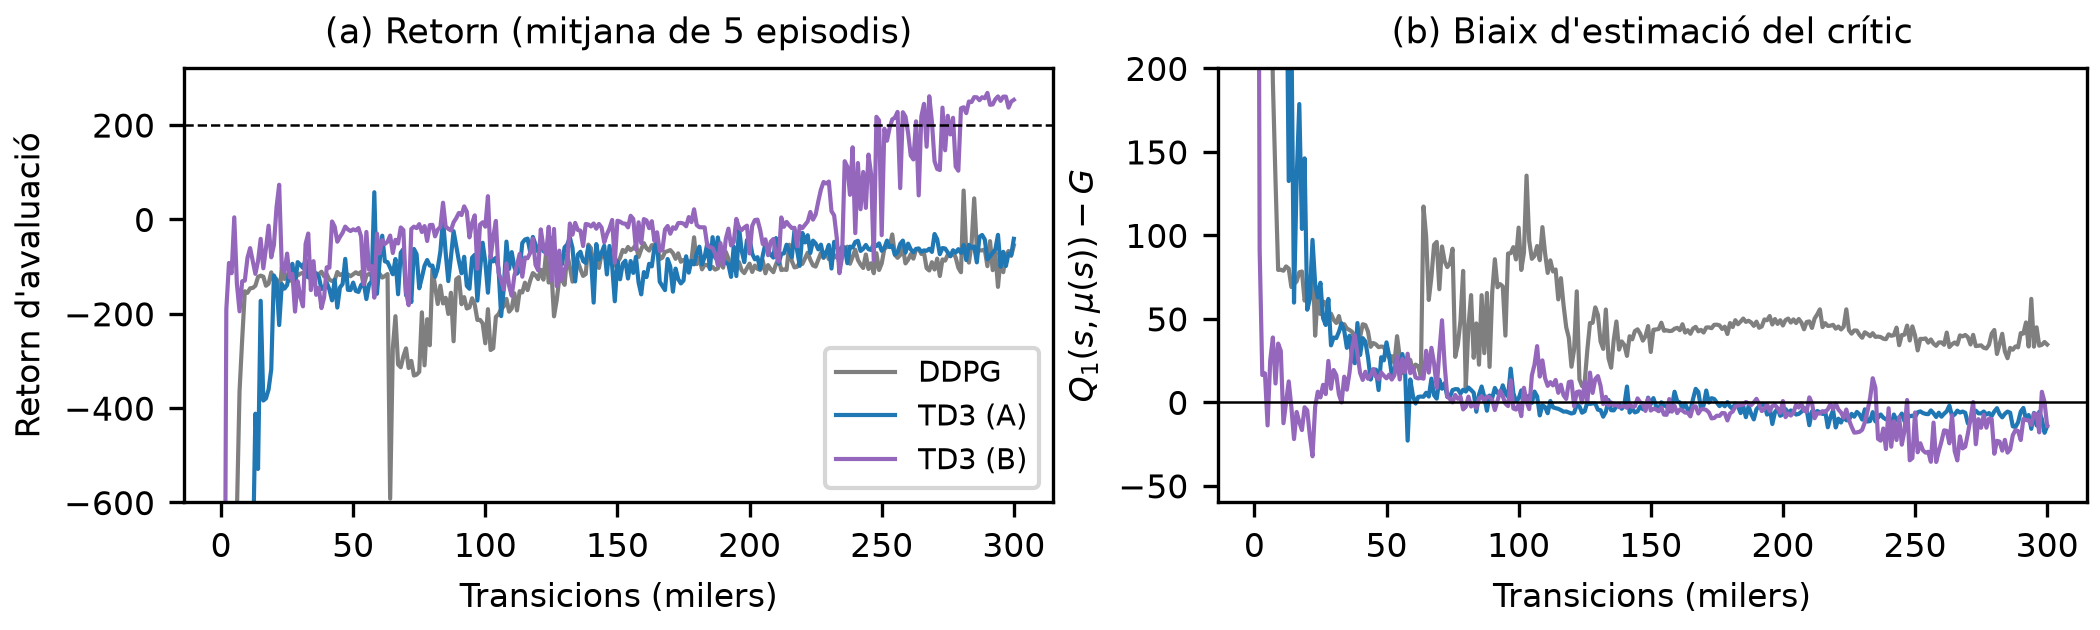
\includegraphics[width=\linewidth]{img/fig_ddpg_td3.png}
  \caption{Comparació exploratòria amb la llavor 0. (a) Retorn d'avaluació, mitjana de 5 episodis deterministes cada 1.000 transicions; l'eix vertical està retallat a −600 (els valors inicials són d'uns −1.440). (b) Biaix $Q_1(s,\mu(s))-G$ als episodis d'avaluació.}
  \label{fig:ddpg}
\end{figure}

A la Figura~\ref{fig:ddpg}, totes dues execucions surten del retorn inicial d'uns −1.440 en poques avaluacions (DDPG supera −200 als 9.000 passos i TD3 als 15.000) i acaben en un nivell semblant: L10 de −83,6 per a DDPG i de −70,3 per a TD3. La diferència clara és al crític: al final, el de DDPG sobreestima el retorn en 40,2 punts de mitjana, mentre que el primer crític de TD3 queda lleugerament per sota ($-10{,}6$), que és la direcció que motiva TD3 \parencite{fujimoto2018}. Amb una sola llavor per algorisme i dos sorolls d'exploració diferents, aquesta comparació no és evidència d'una diferència de rendiment.

\section{Estudi d'ablació: resultats}\label{sec:resultats}

\begin{figure}[htbp]
  \centering
  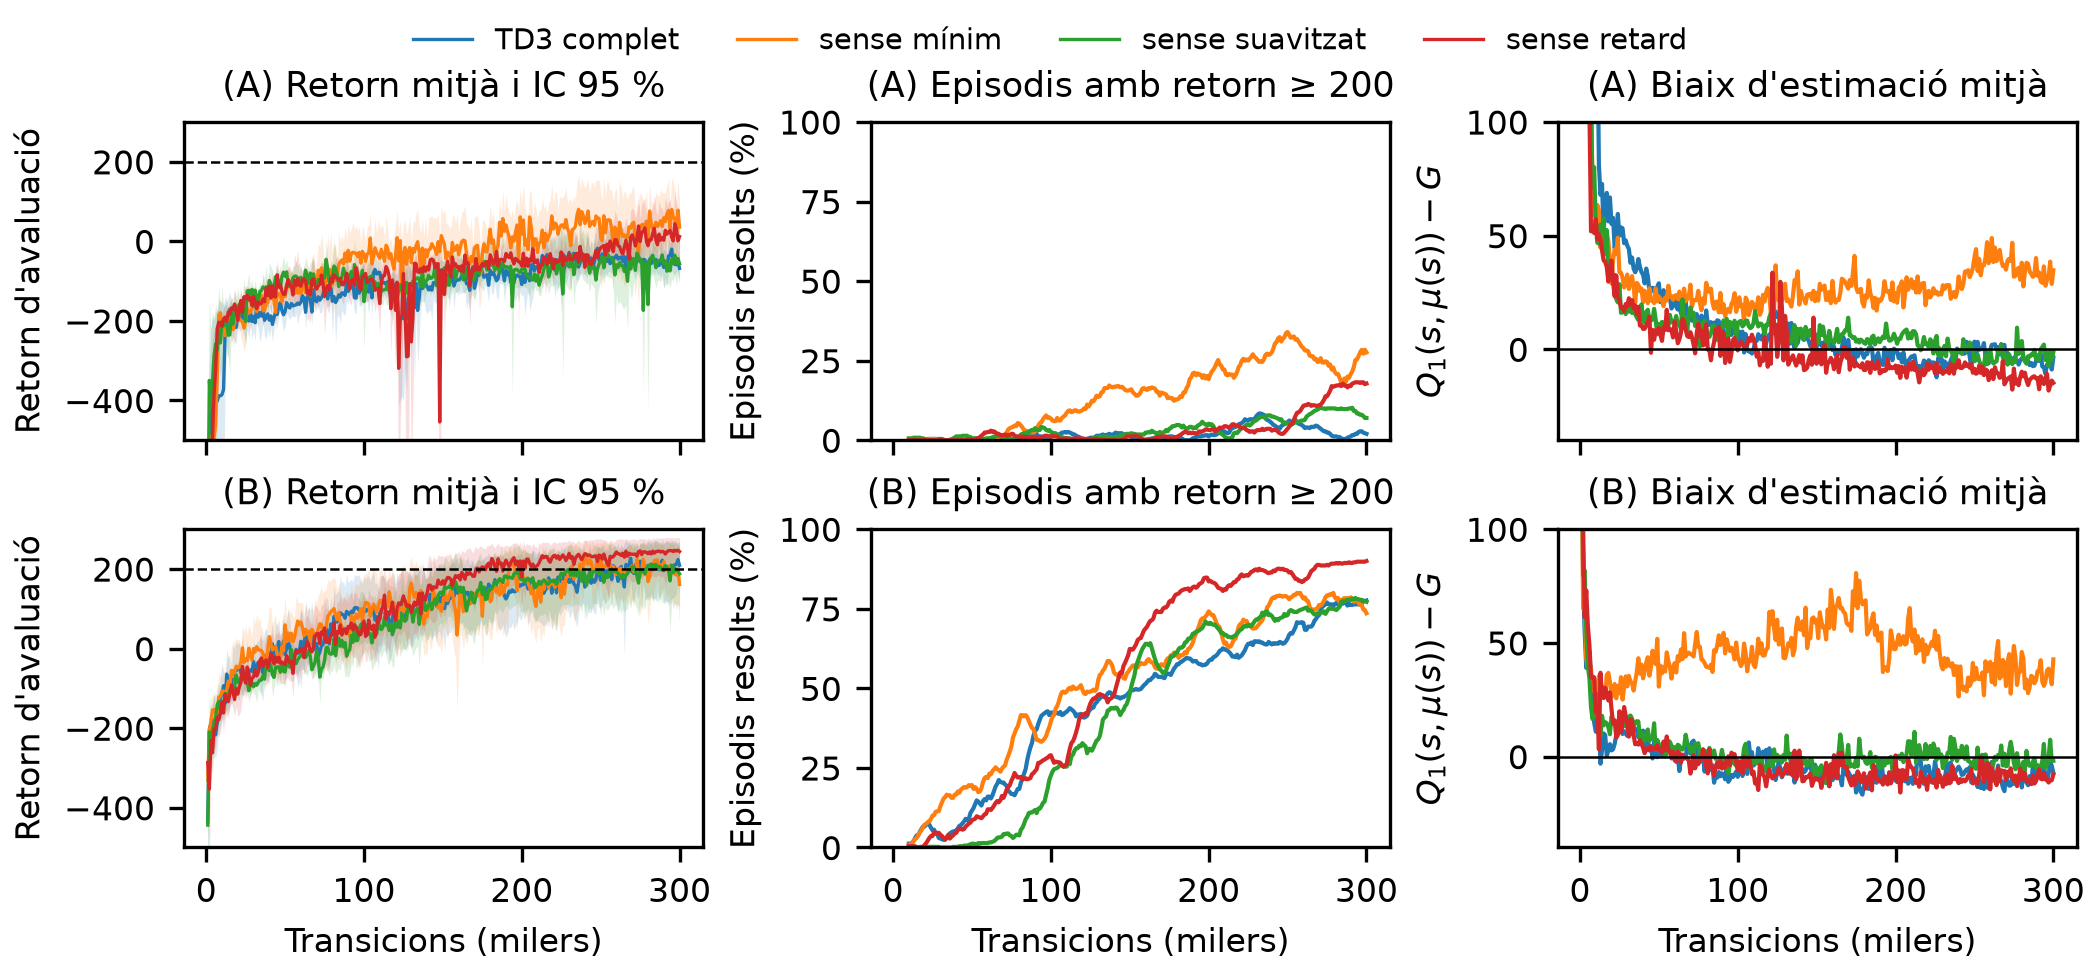
\includegraphics[width=\linewidth]{img/fig_ablacio.png}
  \caption{Ablació de TD3, 10 llavors per variant. (a) Retorn d'avaluació mitjà entre llavors cada 1.000 transicions, amb IC del 95~\% per \emph{bootstrap}; l'eix vertical està retallat a −500. (b) Percentatge d'episodis d'avaluació amb retorn ≥ 200 (mitjana mòbil de 10 avaluacions). (c) Biaix mitjà $Q_1(s,\mu(s))-G$.}
  \label{fig:ablacio}
\end{figure}

\begin{table}[htbp]
  \centering
  \small
  \caption{Ablació, 10 llavors per variant (mitjana ± desviació estàndard). Δ L10: diferència aparellada respecte de TD3 complet; $p$ Holm: test de permutació aparellat exacte amb correcció de Holm. Sobre les últimes 10 avaluacions: Resolts, episodis amb retorn ≥ 200; Truncades, avaluacions amb els cinc episodis truncats a 1.000 passos; Biaix, $Q_1(s,\mu(s))-G$.}
  \label{tbl:ablacio}
  \setlength{\tabcolsep}{2.5pt}
  \begin{tabular}{lrrrrrrr}
    \toprule
    Variant & L10 & AUC/T & Δ L10 [IC 95~\%] & $p$ Holm & Resolts & Truncades & Biaix \\
    \midrule
    TD3 complet & −51,3 ± 45,9 & −115,2 ± 43,5 & --- & --- & 2,0~\% & 65~\% & −6,4 ± 7,5 \\
    Sense mínim & 55,4 ± 110,1 & −45,8 ± 67,0 & +106,6 [27,5, 177,6] & 0,088 & 27,6~\% & 25~\% & +32,2 ± 18,2 \\
    Sense suavitzat & −54,6 ± 95,1 & −95,6 ± 48,4 & −3,4 [−51,1, 55,1] & 0,902 & 7,0~\% & 70~\% & −2,2 ± 13,3 \\
    Sense retard & 19,7 ± 110,5 & −86,8 ± 45,3 & +70,9 [11,2, 142,7] & 0,152 & 17,8~\% & 57~\% & −14,4 ± 11,5 \\
    \bottomrule
  \end{tabular}
\end{table}

Cap variant arriba al llindar de 200 en mitjana, i les corbes de retorn de sense mínim i sense retard encara pugen als 300.000 passos, mentre que la de TD3 complet és gairebé plana des dels 250.000 (Figura~\ref{fig:ablacio}a). La variant sense mínim obté la L10 i l'AUC/T més altes (Taula~\ref{tbl:ablacio}) i supera TD3 complet en 8 de les 10 llavors, amb $p = 0{,}029$ sense corregir i $p = 0{,}088$ amb Holm. La variant sense retard també millora la mitjana en 8 de 10 llavors ($p = 0{,}152$ amb Holm), però la seva mediana (−27,7) queda molt per sota de la mitjana (19,7) perquè dues llavors, amb una L10 de 239,8 i 184,7, concentren la millora. Sense suavitzat, en canvi, no es distingeix de TD3 complet, i amb la correcció de Holm cap diferència és significativa al 5~\%.

La fracció d'episodis resolts separa més les variants (Figura~\ref{fig:ablacio}b). Cap llavor de TD3 complet arriba a resoldre el 50~\% dels episodis, i quatre de sense mínim hi arriben o el superen. La diferència es manté en les cinc condicions inicials d'avaluació: sense mínim en resol entre el 21~\% i el 33~\% de cada condició, i TD3 complet entre el 0~\% i el 5~\%. A canvi, sense mínim és la variant més inestable, amb 73 caigudes de més de 200 punts entre avaluacions consecutives després dels 50.000 passos, per 17 de TD3 complet.

El biaix final (Figura~\ref{fig:ablacio}c) és proper a zero o negatiu a les tres variants que conserven el mínim. L'única que sobreestima és sense mínim, amb un valor proper al de DDPG (secció~\ref{sec:ddpg}). Dins de cada variant, les llavors amb més biaix tendeixen a acabar amb menys retorn: la correlació de Spearman entre el biaix i la L10 va de −0,24 a −0,72 segons la variant (10 llavors cadascuna).

\section{Discussió}\label{sec:discussio}

\subsection{Prova de control}\label{sec:control}

Com que TD3 complet no aterrava amb la configuració A, vam comprovar que no fos per un error d'implementació amb una prova fora del protocol, amb les llavors 0--4. La configuració \emph{td3\_paper} aplica els hiperparàmetres de la taula 3 de \textcite{fujimoto2018}: $\tau = 0{,}005$, taxa d'aprenentatge de $10^{-3}$ a l'actor i als crítics, cap \emph{weight decay}, lots de 100 i 10.000 passos inicials d'accions uniformes. \emph{Sense weight decay} només treu el \emph{weight decay} dels crítics. Amb td3\_paper, la llavor 3 resol l'entorn (269,7 punts i 98~\% d'episodis resolts en una avaluació final de 100 episodis), però les llavors 0, 2 i 4 continuen planejant (entre el 83~\% i el 100~\% d'episodis truncats). Sense \emph{weight decay}, el biaix puja en les cinc llavors (de −4,5 a +26,1 de mitjana), però el 79,8~\% dels episodis finals es trunquen.

\subsection{El planeig}\label{sec:planeig}

A TD3 complet amb la configuració A, el 65~\% de les últimes avaluacions tenen els cinc episodis truncats als 1.000 passos (Taula~\ref{tbl:ablacio}): el mòdul no s'estavella ni arriba a repòs. Com que les xarxes finals de l'estudi principal no es van desar, vam mesurar el comportament amb les de la prova de control (20 episodis per a cadascuna de les 10 execucions). Se'n van truncar 143 de 200. En els últims 200 passos, el mòdul era per sobre del terra el 88~\% del temps (\emph{y} mitjana de 0,38; 0 és l'alçada de la plataforma). Les dues potes tocaven terra l'1,6~\% del temps i el motor principal estava encès en el 73~\% dels passos.

La recompensa de LunarLander fa que aquest comportament sigui estable \parencite{gymnasium}. Cada pas amb el motor principal encès costa fins a 0,3 punts, i planejar fins al límit acaba en un retorn moderadament negatiu (−42,4 de mitjana en aquests episodis), mentre que un aterratge fallit suma −100. Aterrar dona +100, però abans cal passar per estats propers al terra en què una acció dolenta porta al xoc. Si aquests estats apareixen poc a la memòria de repetició i el crític els valora malament, és d'esperar que l'actor, que segueix el gradient de $Q_1$, es quedi planejant. Les dades no permeten verificar aquest mecanisme directament.

La configuració B fa el planeig molt menys freqüent, però no l'elimina: de les 8 execucions de B que resolen menys del 50~\% dels episodis finals, 7 en tenen més de la meitat truncats. Els quatre canvis de B es van aplicar junts i no podem dir quin evita el planeig. td3\_paper, que en comparteix dos ($\tau = 0{,}005$ i cap \emph{weight decay}), només aterra en una de cinc llavors.

\subsection{Què canvia cada mecanisme}\label{sec:mecanismes}

El mínim és l'únic mecanisme amb un efecte clar sobre el crític: sense ell apareix la sobreestimació en les dues configuracions. Treure'l també fa l'aprenentatge més inestable: les caigudes de més de 200 punts entre avaluacions consecutives després dels 50.000 passos passen de 17 a 73 a la configuració A i de 13 a 34 a la B ($p = 0{,}031$ i $p = 0{,}016$, tests exactes sense corregir d'una anàlisi exploratòria). A la configuració B, a més, la sobreestimació va lligada al fracàs: a sense mínim, la correlació de Spearman entre el biaix i la L10 és de −0,90, i les tres llavors amb més biaix són les tres que fallen.

L'efecte del mínim sobre el retorn, en canvi, no és el mateix a les dues configuracions: a A, treure'l és el canvi que més millora el retorn, i a B no el millora. Tot i així, la diferència entre els dos efectes (−120,4 de L10, $p = 0{,}107$) no és significativa amb deu llavors. El mínim, per si sol, tampoc no provoca el planeig: TD3 complet el conserva a la configuració B i només hi fallen 2 de 10 llavors.

El suavitzat no té cap efecte clar en el retorn, i sense ell el biaix només puja lleugerament (+5,3 a B, $p = 0{,}047$ sense corregir). Treure el retard, que duplica les actualitzacions de l'actor, millora la mitjana a A i a B, sense significació: a A la millora depèn de dues llavors, i a B hi aterren 9 de 10 llavors, per 8 de TD3 complet.

\subsection{Limitacions}\label{sec:limitacions}

L'ablació, amb deu llavors, no pot detectar diferències de la mida observada, perquè el resultat de cada variant depèn sobretot de quantes llavors fallen. Les xarxes de l'esquelet usen LayerNorm, i l'enunciat parla de \emph{batch normalization}. El biaix es mesura sobre els estats de cada política i per a $\mu$, mentre que el crític aprèn el valor de la política suavitzada.

\section{Conclusions}\label{sec:conclusions}

Amb la configuració recomanada pel professor, TD3 complet resol LunarLander en mitjana dins de $T = 300.000$ transicions, i 8 de les 10 llavors resolen més del 75~\% dels episodis finals. Amb la de l'enunciat, cap variant el resol en mitjana i el mòdul tendeix a planejar. En les dues configuracions, treure el mínim fa aparèixer una sobreestimació semblant a la de DDPG i un aprenentatge més inestable. El seu efecte sobre el retorn no és consistent entre configuracions, i el suavitzat i el retard no tenen cap efecte clar. El pas següent seria separar els quatre canvis de B per saber quin evita el planeig.


\printbibliography

% Anexos
% \appendix
% \input{secciones/A-anexo}

\end{document}
